\documentclass[main.tex]{subfiles}
\begin{document}



\section{Hausdorffmetriek}
\label{sec:hausdorffmetriek}

\begin{de}
  Voor een niet-lege deelverzameling $A$ van $\mathbb{R}^{p}$ en een $r\in \mathbb{R}^{+}$ definie\"eren we de $r$-omhullende $[A]_{r}$ van $A$ als volgt:
  \[ [A]_{r} = \{r \in \mathbb{R}^{p} \mid \exists a \in A:\ d(x,a) \le r \} \]
  Hierin staat $d$ voor de gewone euclidische metriek.
\end{de}

\begin{de}
  Noteer met $\mathcal{F}$ de verzameling van niet-lege gesloten en begrensde deelverzamelingen van $\mathbb{R}^{p}$.
  \[ \mathcal{F} = \{ A \mid A \subseteq \mathbb{R}^{p}, A \text{ is gesloten en begrensd } \} \]
\end{de}

\begin{de}
  We defini\"eren de \term{Hausdorffafstand} $h(F,G)$ tussen twee deelverzamelingen $F,G \in \mathcal{F}$ als volgt:
  \[ h(F,G) = \inf\{ r\in \mathbb{R}^{+} \mid F \subseteq [G]_{r} \text{ en } G \subseteq [F]_{r} \} \]
\end{de}

\begin{blem}
  \label{lem:omhullenden-in-elkaar}
  Zij $A \subseteq \mathbb{R}^{p}$ en $r,s\in\mathbb{R}^{+}$ met $r\ge s \ge 0$.
  \[ [A]_{s} \subseteq [A]_{r} \]

  \begin{proof}
    Dit volgt meteen uit de definitie:
    Kies een $x\in [A]_{s}$, dan bestaat er een $a\in A$ zodat $d(x,a) \le s$ geldt.
    Omdat $r \ge s$ geldt, geldt ook $d(x,a) \le r$ en dus zit $x$ ook in $[A]_{r}$.
  \end{proof}
\end{blem}

\begin{vb}
  De Hausdorffafstand tussen een (vol) gesloten vierkant en zijn omschreven cirkelschijf is gegeven als $\frac{(\sqrt{2}-1)z}{2}$.
  Hierin is $z$ de zijde van het vierkant.

  \begin{proof}
    Beschouw een vierkant $V$ met zijde $z$ en middelpunt $p\in \mathbb{R}^{2}$.
    Merk op dat de omschreven cirkelschijf $C$ hetzelfde middelpunt en straal $r=\frac{z}{\sqrt{2}}$ heeft.
    \begin{figure}[H]
        \centering
        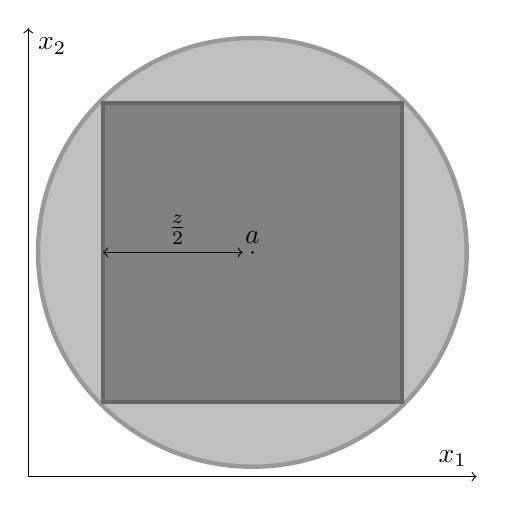
\begin{tikzpicture}
          \begin{axis}[ 
            ticks=none,
            axis lines = middle,
            axis line style={->},
            ymin=0, ymax=3,
            xmin=0, xmax=3,
            xlabel={$x_{1}$},
            ylabel={$x_{2}$},
            axis equal image,
            disabledatascaling
            ]
            \filldraw [ultra thick,fill=black!25!white, draw=black!40!white] (1.5,1.5) circle [radius=sqrt(2)+0.02];
            \filldraw[ultra thick,fill=black!50!white, draw=black!60!white] (0.5,2.5) -- (2.5,2.5) -- (2.5,0.5) -- (0.5,0.5) -- cycle;
            \fill [fill=black] (1.5,1.5) circle [radius=0.01];
            \draw (1.5,1.6) node {$a$};
            \draw (1.5,1.5) node {} edge[<->] (0.5,1.5);
            \draw (1,1.65) node {$\frac{z}{2}$};
          \end{axis}
        \end{tikzpicture}
      \end{figure}
    Voor elke omhullende van de circkel zit het vierkant erin.
    We zoeken dus een de kleinste omhullende van het vierkant dat ook de cirkel omhult.
    Kies $f = \frac{(\sqrt{2}-1)z}{2}$.
    \begin{klad}
      Dit is de afstand tussen een uiterste punt van de cirkel en het dichtstbijzijnde punt op de rand van het vierkant.
      Intu\"itief zou het duidelijk moeten zijn dat dit de Hausdorffaffstand zal zijn.
    \end{klad}
    Beschouw $V_{[f]}$ en kies een willekeurig punt $x$ in de cirkelschijf $C$.
    Er geldt dat $\|x\| < r$ en kies $y = x\frac{\left\|\frac{z}{2}\right\|}{\|r\|}$.
    $y$ ligt dan binnnen $V$\waarom
    Er geldt bovendien:
    \[ \|x-y\| = \|x\| \left|1-\frac{z}{r}\right| \le r - \frac{z}{2} = f \]
    $x$ ligt dus binnen de $f$-omhullende van $V$.
    Er rest ons nog te bewijzen dat $h(C,V)$ zeker niet kleiner is dan $f$.
    Bechouw de rechte door het middelpunt van het vierkant en het midden van een zijde van het vierkant.
    Het is duidelijk dat het dichtste punt $s$ van $C$ tot $V$ het midden $m$ van de zijde van het vierkant is.
    Deze afstand is $f$.
    Als $h(C,V)$ moet dus minstens $f$ bedragen.
  \end{proof}
\end{vb}

\begin{blem}
  Zij $A \subseteq \mathbb{R}^{p}$ en $r,s\in\mathbb{R}^{+}$:
  \[ \left[ [A]_{r}\right]_{s} \subseteq [A]_{r+s} \]

  \begin{proof}
    Kies een $x\in \left[[A]_{r}\right]_{s}$, dan bestaat er een $b\in [A]_{r}$ als volgt:
    \[ d(x,b) \le s \]
    Omdat $b$ in $[A]_{r}$ zit, bestaat er ook een $c\in A$ als volgt:
    \[ d(b,c) \le r \]
    We gebruiken nu de driehoeksongelijkheid:
    \[ d(x,c) \le d(x,b) + d(b,c) \le r + s \]
    $x$ behoort dus tot $[A]_{r+s}$.
  \end{proof}
\end{blem}

\begin{blem}
  Zij $F,G \in \mathcal{F}$ en $r=h(F,G)$.
  \[ F \subseteq [G]_{r} \text{ en } G \subseteq [F]_{r} \]

  \begin{proof}
    Kies een willekeurige $x\in F$.
    Omdat $r = h(F,G)$ geldt, zal volgens de definitie van $h$ het volgende gelden:\lemref{lem:omhullenden-in-elkaar}
    \[ F \subseteq [G]_{r+\frac{1}{n}}\]
    Er bestaat dus een rij punten $(y_{n})_{n}$ in $G$ met de volgende eigenschap:
    \[ \forall n \in \mathbb{N}:\ d(x,y_{n}) \le r + \frac{1}{n} \]
    Omdat $G$ gesloten en begrensd is, bestaat er een deelriij $(y_{n_{k}})_{k}$ die convergeert naar een $y\in G$.\stref{st:in-rp-gesloten-en-begrensd-itv-rijen}
    Voor deze $y$ zal $d(x,y) \le r$ gelden.
    We vinden dus dat $x$ in $[G]_{r}$ zit.
    $F$ moet dus een deel zijn van $[G]_{r}$ en omgekeerd is de redenering hetzelfde met de namen $F$ en $G$ omgewisseld.
  \end{proof}
\end{blem}

\begin{pr}
  De Hausdorffafstand $h$ is een metriek die $\mathcal{F},h$ een metrische ruimte maakt.

  \begin{proof}
    We gaan de eigenschappen van een metrische ruimte na.
    \begin{itemize}
    \item $\forall F,G\in \mathcal{F}:\ h(F,G) \ge 0$: Dit volgt meteen uit de definitie.
    \item $\forall F,G\in \mathcal{F}:\ h(F,G) = 0 \Leftrightarrow F = G$: Idem
    \item $h$ is symmetrisch: Dit zit vervat in de definitie.
    \item $h$ voldoet aan de driehoeksongelijkheid.
      Kies 3 elementen $F$, $G$ en $H$ uit $\mathcal{F}$.
      Noem $s=h(F,G)$ en $t=(G,H)$.
      Meteen vinden we het volgende:
      \[ G \subseteq [H]_{t} \quad\text{ en }\quad F \subseteq [G]_{s} \subseteq \left[[H_{t}]\right]_{s} \subseteq [H_{t+s}] \]
      Analoog vinden we $H \subseteq [F]_{t+s}$ en bijgevolg $h(F,H) \le s+t$.\needed
    \end{itemize}
  \end{proof}
\end{pr}

\begin{opm}
  Het is belangrijk dat de deelverzamelingen waartussen we de afstand meten gesloten en begrensd zijn.
  Stel immers dat \'e\'en ervan niet begrensd zou zijn, dan bestaat de Hausdorffafstand niet.
  Een $r$-omhulling heeft immers een eindige $r$ nodig om zinvel te zijn.
  Stel anderzijds dat de verzamelingen niet gesloten zouden zijn, dan bestaat het supremem in de definitie niet noodzakelijk.
\end{opm}

\begin{st}
  \label{st:rp-als-deel-van-f}
  \[ \forall x,y \in \mathbb{R}^{p}:\ h(\{x\},\{y\}) = d(x,y) \]
\end{st}

\begin{opm}
  We kunnen $\mathbb{R}^{p},d$ dus als deelruimte van $\mathcal{F},h$ via de inbedding $\mathfrak{i}$ als volgt:
  \[ \mathfrak{i}:\ \mathbb{R}^{p} \rightarrow \mathcal{F}:\ x \mapsto \{x\} \]
\end{opm}

\begin{vb}
  Beschouw $F_{1} = B\interval{x_{1}}{r_{1}}$ en $F_{2}= B\interval{x_{2}}{r_{2}}$.

\extra{bewijs: $h(F_{1},F_{2}) = d(x_{1},x_{2}) + |r_{1}-r_{2}|$.}
\end{vb}

\extra{voorbeelden van HDafstandberekeningen}

\begin{st}
  Een rij gesloten bollen $(B_{n})_{n}$ in $\mathbb{R}^{p}$ met middelpunten $x_{n}$ en stralen $r_{n}$ zal voor de Hausdorffmetriek convergeren naar een gesloten bol $B$ met middelpunt $x$ en straal $r$ als en slechts als $\lim_{n\rightarrow +\infty}x_{n}=x$ en $\lim_{n\rightarrow +\infty}r_{n} = r$ gelden.
\extra{bewijs}
\begin{klad}
\begin{proof}
  \begin{lem}
    $\forall r,s \in \mathbb{R}^{+}:\ \left[B\interval{x}{r}\right]_{s} = B\interval{x}{r+s}$
  \end{lem}

  \begin{lem}
    $\forall r\in \mathbb{R}^{+}:\ B\interval{x}{r} \subseteq B\interval{y}{r+\|x-y\|}$
  \end{lem}
  Gevalsonderscheid.
\end{proof}
\end{klad}
\end{st}

\begin{st}
  $(n)_{n}$ in $\mathbb{R}$ is voor de gewone metriek geen Cauchyrij maar wel voor de $d_{2}$-metriek.
\extra{bewijs}
\extra{wat met de $d_1$-metriek?}
\end{st}

\begin{vb}
  Beschouw de niet-lege, gesloten, begrensde deelverzameling $F_{n}$ van $\mathbb{R}$ als volgt voor een $n\in \mathbb{N}_{0}$.
  \[ F_{n} = \{0,1\} \cup \left\{ \frac{i}{n} \ \middle|\ i \in \mathbb{N}, 0 \le \frac{i}{n} \le 1 \right\} \]
  De rij $(F_{n})_{n}$ convergeert volgens de Hausdorffmetriek.
  \begin{proof}
    \begin{klad}
      Om een idee te krijgen van hoe $F_{n}$ eruit ziet tekent u best een paar instanties.
      U ziet dan meteen dat $(F_{n})_{n}$ zal convergeren.

      \begin{figure}[H]
        \centering
        \foreach \n in {1,...,20} {
          \begin{tikzpicture}
            \foreach \l in {0,...,\n} {
              \node(\n\l) at (\l/\n,0) {\textbullet};
            }
          \end{tikzpicture}
        }
      \end{figure}
      Het ziet ernaar uit dat $(F_{n})_{n}$ naar $\interval{0}{1}$ zal convergeren.
      Het kan van pas komen om de Hausdorffafstand van $F_{n}$ tot $\interval{0}{1}$ voor een paar getallen $n\in \mathbb{N}_{0}$ te berekenen.

      \begin{figure}[H]
        \centering
        \foreach \n in {1,...,9} {
          \begin{tikzpicture}
            \foreach \l in {0,...,\n} {
              \fill [thick,fill=black!25!white,opacity=0.2] (\l/\n,) circle [radius=1/(2*\n)];
              \node(\n\l) at (\l/\n,) {\textbullet};
            }
          \end{tikzpicture}
        }
      \end{figure}
      \[
      \begin{array}{|c|c|c|c|c|c|c|c|}
        \hline
        n & 1 & 2 & 3 & 4 & 5 & 6 & i\\
        \hline
        H(F_{n},L) & \frac{1}{2} & \frac{1}{4} & \frac{1}{6} & \frac{1}{8} & \frac{1}{10} & \frac{1}{12} & \frac{1}{2i}\\
        \hline
      \end{array}
      \]
      Vanaf de derde $F_{n}$ zou het patroon duidelijk moeten zijn.
    \end{klad}
    Merk op dat de Hausdorffafstand tussen $F_{n}$, voor een gegeven $n\in \mathbb{N}_{0}$ en $\interval{0}{1}$ steeds $\frac{1}{2n}$ meet.
    Kies willekeurig een $\epsilon \in \mathbb{R}_{0}^{+}$ en noem $n_{0}= \frac{1}{2\epsilon}$.
    Kies nu willekeurig een $n\in\mathbb{N}$,strikt groter dan $n_{0}$.
    \[ h(F_{n},\interval{0}{1}) = \frac{1}{2n} < \frac{1}{2n_{0}} = \frac{2\epsilon}{2} = \epsilon \]
    $(F_{n})_{n}$ convergeert dus naar $\interval{0}{1}$ voor de Hausdorffmetriek.
  \end{proof}
\end{vb}

\begin{vb}
  \label{vb:ttt-2-2014-1}
  \examenvraag{TTT II 2014}
  Beschouw de niet-lege, gesloten, begrensde, deelverzameling $F_{n}$ van $\mathbb{R}^{2}$ als volgt voor een $n\in \mathbb{N}_{0}$.
  \[ F_{n} = \left\{ \left(\frac{k}{n},\frac{t}{n}\right) \middle| t,k \in \{0,\dotsc,n\} \right\} \]
  De rij $(F_{n})_{n}$ convergeert volgens de Hausdorffmetriek.

  \begin{proof}
    Merk op dat we inderdaad over de Hausdorffafstand kunnen spreken omdat de $F_{n}$ niet leeg, gesloten en begrensd zijn.
    \begin{klad}
      Om een idee te krijgen van hoe $F_{n}$ eruit ziet zal u waarschijnlijk minstens twee intanties ervan moeten tekenen.
      Wanneer we die verzamelingen tekenen krijgen we een idee van de convergentie van $F_{n}$ en bovendien van de limiet.

      \begin{figure}[H]
        \centering
        \foreach \n in {1,...,20} {
          \begin{tikzpicture}
            \foreach \k in {0,...,\n} {
              \foreach \l in {0,...,\n} {
                \node(\n\k\l) at (\k/\n,\l/\n) {\textbullet};
              }
            }
          \end{tikzpicture}
        }
      \end{figure}
      Het ziet ernaar uit dat de limiet er als volgt zal uitzien:
      \[ L = \{ (x,y) \mid x,y\in\interval{0}{1} \} \]
      Het kan van pas komen om de Hausdorffafstand van $F_{n}$ tot $L$ voor een paar getallen $n\in \mathbb{N}_{0}$ te berekenen.

      \begin{figure}[H]
        \centering
        \foreach \n in {1,...,9} {
          \begin{tikzpicture}
            \foreach \k in {0,...,\n} {
              \foreach \l in {0,...,\n} {
                \fill [thick,fill=black!25!white,opacity=0.2] (\k/\n,\l/\n) circle [radius=sqrt(2)/(2*\n)];
                \node(\n\k\l) at (\k/\n,\l/\n) {\textbullet};
              }
            }
          \end{tikzpicture}
        }
      \end{figure}
      \[
      \begin{array}{|c|c|c|c|c|c|c|c|}
        \hline
        n & 1 & 2 & 3 & 4 & 5 & 6 & i\\
        \hline
        H(F_{n},L) & \frac{\sqrt{2}}{2} & \frac{\sqrt{2}}{4} & \frac{\sqrt{2}}{6} & \frac{\sqrt{2}}{8} & \frac{\sqrt{2}}{10} & \frac{\sqrt{2}}{12} & \frac{\sqrt{2}}{2i}\\
        \hline
      \end{array}
      \]
    \end{klad}
    Merk op dat de Hausdorffafstand tussen $F_{n}$, voor een gegeven $n\in \mathbb{N}_{0}$, en de verzameling $L$ als volgt steeds $\frac{\sqrt{2}}{2n}$ meet.
    \[ L = \{ (x,y) \mid x,y\in\interval{0}{1} \} \]
    Kies willekeurig een $\epsilon \in \mathbb{R}_{0}^{+}$ en noem $n_{0} = \frac{1}{\sqrt{2}\epsilon}$.
    Kies nu willekeurig een $n\in \mathbb{N}$, strikt groter dan $n_{0}$.
    \[ h(F_{n},L) = \frac{\sqrt{2}}{2n} < \frac{\sqrt{2}}{2n_{0}} = \frac{\sqrt{2}^{2}\epsilon}{2} = \epsilon \]
    $(F_{n})_{n}$ convergeert dus naar $L$ voor de Hausdorff metriek.
  \end{proof}
\end{vb}

\begin{opm}
  Het patroon van de twee bovenstaande voorbeelden kunnen we voorzetten naar $\mathbb{R}^{p}$.
  Daar is de Hausdorffafstand tussen $F_{n}$ en $L$ dan $\frac{\sqrt{p}}{2n}$ en convergeert $(F_{n})_{n}$ naar een $p$-dimensionale gesloten cubus.
\end{opm}


\end{document}

%%% Local Variables:
%%% mode: latex
%%% TeX-master: t
%%% End:
